\section{Related Work}
\label{sec:related}

\begin{figure}[t!]
\begin{minipage}{\textwidth}
  \centering
  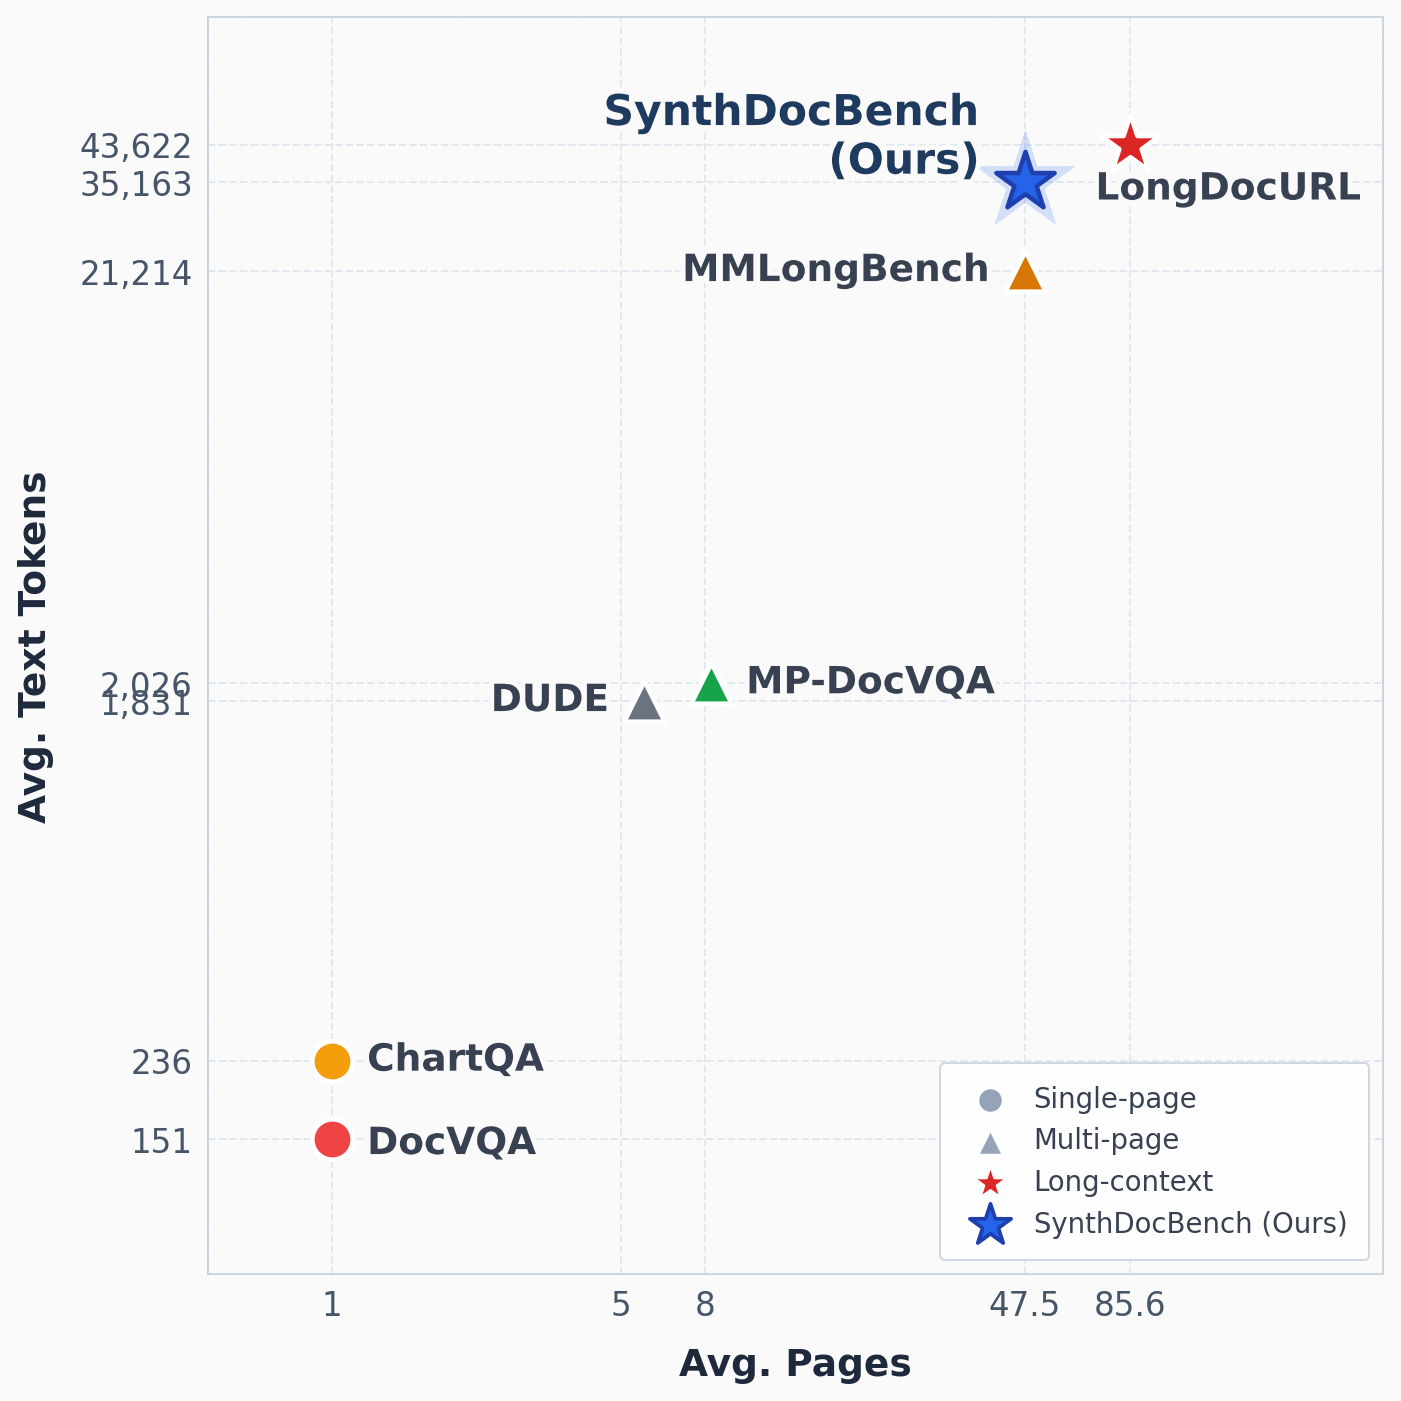
\includegraphics[width=0.55\textwidth]{images/benchmark_plot.png}
\end{minipage}

\vspace{14pt}

\begin{minipage}{\textwidth}
  \centering
  \footnotesize
  \resizebox{\textwidth}{!}{%
  \begin{tabular}{@{}lcccc@{}}
  \toprule
  \textbf{Benchmark} & \textbf{Scope} & \textbf{Avg.\ Context} & \textbf{\#Docs/Charts} & \textbf{\#Questions} \\
  \midrule
  \rowcolor{gray!15} \multicolumn{5}{c}{{Chart Benchmarks}} \\
  \midrule
  ChartQA \citep{masry2022chartqa}               & Isolated charts   & 1 chart       & 21,953    & 32,701 \\
  ChartQAPro \citep{masry2025chartqapro}         & Isolated charts   & 1 chart       & 1,341     & 1,948  \\
  ChartGalaxy \citep{li2025chartgalaxy}          & Isolated charts   & 1 chart       & 1,763,189 & ---    \\
  VisuLogic \citep{zhang2025visulogic}           & Isolated images   & 1 image       & 1,000     & 1,000  \\
  ChartMuseum \citep{xu2025chartmuseum}          & Isolated charts   & 1 chart       & 928       & 1,162  \\
  MultiChartQA \citep{zhu2025multichartqa}       & Multi-chart       & 2--3 charts   & 655       & 944    \\
  \midrule
  \rowcolor{gray!15} \multicolumn{5}{c}{{Document VQA Benchmarks}} \\
  \midrule
  DocVQA \citep{mathew2021docvqa}                & Single-page docs  & 1 page        & 12,767    & 50,000 \\
  MP-DocVQA \citep{tito2023hierarchical}         & Multi-page docs   & $\leq$20 pages & ---      & 46,000 \\
  SlideVQA \citep{tanaka2023slidevqa}            & Multi-page docs   & $\sim$20 pages & 2,619    & 14,500 \\
  MMLongBench-Doc \citep{ma2024mmlongbenchdoc}   & Multi-page docs   & 47.5 pages    & 135       & 1,082  \\
  LongDocURL \citep{deng2025longdocurl}          & Multi-page docs   & $\sim$83 pages & 396      & 2,325  \\
  M-LongDoc \citep{chia2024mlongdoc}             & Multi-page docs   & $>$200 pages  & ---       & 851    \\
  MMLongBench \citep{wang2025mmlongbench}        & Multi-page docs   & 8K--128K tokens & 13,331  & ---    \\
  \midrule
  
\includegraphics[width=0.8em]{images/icon2.png} \textbf{\textsc{SynthDocBench}} & \textbf{Multi-page docs} & \textbf{Avg.\ 51.1 pages} & \textbf{200 / 3,340} & \textbf{1,788} \\
  \bottomrule
  \end{tabular}
  }
  % \captionof{table}{Benchmarks in chart reasoning and long-context document understanding. ChartGalaxy and MMLongBench do not report \#Questions; MP-DocVQA and M-LongDoc do not report doc counts.}
\end{minipage}
\vspace{-6pt}
\caption{\textbf{Landscape of benchmarks} 
Top: benchmark comparison by average document length (pages) and average textual context (tokens). SynthDocBench occupies a unique region with both long multi-page context and high textual density.
Bottom: comparison with existing chart and document VQA benchmarks. 
Prior benchmarks typically isolate either charts or long documents, whereas \textbf{\textsc{SynthDocBench}} is designed to study their intersection under long contexts.}
\label{fig:related_benchmarks}
\end{figure} % contains fig also

\paragraph{Charts and Visual Reasoning.}
Chart understanding has been evaluated primarily in isolation from document context. ChartQA~\citep{masry2022chartqa} established the standard evaluation setup for chart-oriented VQA, now approaching saturation. ChartQAPro~\citep{masry2025chartqapro} addresses this through harder, more diverse real-world charts, exposing over 30 percentage points of degradation for models that saturate ChartQA, though it retains the isolated-image setting. ChartGalaxy~\citep{li2025chartgalaxy} demonstrates that programmatic generation can yield million-scale synthetic diversity spanning 75 chart types and 330 stylistic variations, providing a methodological precedent for \synthdocbench{}'s synthetic approach. VisuLogic~\citep{zhang2025visulogic} and ChartMuseum~\citep{xu2025chartmuseum} probe fine-grained logical and perceptual reasoning over isolated charts, while MultiChartQA~\citep{zhu2025multichartqa} extends this to simultaneous multi-chart reasoning. Collectively, these benchmarks establish that chart understanding is far from solved, yet none evaluate charts within the document contexts where they naturally occur and where interpretation requires engagement with surrounding text, tables, and figures.


\paragraph{Long-Context Multimodal Benchmarks.}
Early long-context evaluation focused on needle-in-a-haystack retrieval~\citep{wang2024mmniah}, which provides insufficient difficulty ceilings for frontier models and correlates poorly with downstream reasoning performance~\citep{wang2025mmlongbench}. Document-centric benchmarks have progressed from single-page evaluation via DocVQA~\citep{mathew2021docvqa} through multi-page extensions including MP-DocVQA~\citep{tito2023hierarchical} and SlideVQA~\citep{tanaka2023slidevqa}, though both are constrained to roughly twenty pages and principally assess span extraction. MMLongBench-Doc~\citep{ma2024mmlongbenchdoc} was the first benchmark targeting long PDF comprehension with interleaved visual content, and MMLongBench~\citep{wang2025mmlongbench} extended this framework to five task categories spanning up to 128K tokens. LongDocURL~\citep{deng2025longdocurl} and M-LongDoc~\citep{chia2024mlongdoc} advance the state of the art through cross-element localisation and open-ended responses, but both prioritize breadth of coverage over diagnostic decomposition. 
% Neither constructs questions requiring joint reasoning over multiple charts and textually distributed evidence across distant pages. 
\synthdocbench{} is distinguished by its explicitly diagnostic design: document length, page depth, modality composition, and question type are varied as independent axes, with charts and figures foregrounded as primary reasoning targets whose interpretation requires engagement with arbitrarily distant contextual evidence.

\paragraph{Vision-Language Models for Document Understanding.}
Recent vision-language models have made single-page document QA increasingly saturated: frontier systems such as Qwen3-VL~\citep{bai2025qwen3} and InternVL3.5~\citep{wang2025internvl3} now approach ceiling performance on DocVQA, so these benchmarks provide limited diagnostic separation among leading models. In contrast, long-context visual document reasoning remains substantially harder: the best reported results on MMLongBench-Doc remain far below single-page performance.\footnote{\url{https://huggingface.co/spaces/OpenIXCLab/mmlongbench-doc}, accessed March 2026.} This gap suggests that failures are driven by properties that emerge in multi-page settings e.g., long-range dependency tracking, retrieval over dispersed evidence, yet current evaluations do not isolate which document factors are most responsible. Figure~\ref{fig:related_benchmarks} situates document VQA benchmarks by average document length (pages) and average token count. Single-page benchmarks (DocVQA, ChartQA) lie in the bottom-left, whereas multi-page benchmarks shift toward higher length and token regimes. \synthdocbench{} lies near the frontier along both axes, comparable to LongDocURL in page count and substantially denser in tokens than MMLongBench, while using controlled synthetic documents and requiring retrieval and reasoning over multi-modal evidence across multiple pages.

% \paragraph{Vision-Language Models for Document Understanding.}
% % The rapid capability growth of VLMs motivates the need for more diagnostic evaluation. On DocVQA, frontier models including 
% Qwen3-VL~\citep{bai2025qwen3} and InternVL3.5~\citep{wang2025internvl3} approach or exceed 95\% on DocVQA, rendering single-page evaluations largely uninformative for discriminating among leading systems. Performance on long-context benchmarks remains considerably more constrained, with the strongest model on MMLongBench-Doc achieving 57\%\footnote{\url{https://huggingface.co/spaces/OpenIXCLab/mmlongbench-doc}, accessed March 2026}. This gap between single-page and long-context performance indicates that long-context visual document reasoning remains a substantively unsolved problem, and that existing benchmarks provide insufficient diagnostic signal to identify the specific document properties and reasoning demands responsible for observed failures.

% Figure~\ref{fig:related_benchmarks} visualizes the landscape of document VQA benchmarks along two axes: average document length (pages) and average token count per document. Single-page benchmarks (DocVQA, ChartQA) occupy the bottom-left, while multi-page benchmarks cluster toward the right. \synthdocbench{} sits at the frontier of both axes among multi-page benchmarks --- comparable to LongDocURL in page count and substantially richer in token density than MMLongBench --- while being the only benchmark in this space built entirely from controlled synthetic documents and requiring retrieval and reasoning over multiple modalities over multiple pages for long-context question answering.
